\documentclass[runningheads]{llncs}

\usepackage[T1]{fontenc}
\usepackage{graphicx}
\usepackage{amsmath,amssymb}
\usepackage{booktabs}
\usepackage{array}
\usepackage{multirow}
\usepackage{url}
\usepackage{orcidlink}

% Tighten floats and spacing to reduce page count
\renewcommand{\floatsep}{4pt}
\renewcommand{\textfloatsep}{6pt}
\renewcommand{\intextsep}{6pt}
\setlength{\belowcaptionskip}{2pt}
\setlength{\abovetopsep}{2pt}

\begin{document}

\title{
A Hybrid Quantum--Classical State-Space Framework for Cyber-Defense Optimization:
LQR-to-QUBO Formulation and IBM Quantum Validation%
\thanks{\raggedright Source code available at:
\url{https://github.com/Greghori101/quantum-cyber-defense-optimization}}
}

\titlerunning{Hybrid Quantum--Classical Cyber-Defense Optimization}

\author{
Hadji Ibrahim\orcidlink{0009-0009-0689-095X}\inst{1} \and
Souala Elhoussine\orcidlink{0009-0009-2451-7788}\inst{1} \and
Mohamed Guerroumi\orcidlink{0000-0001-9998-0608}\inst{1} \and
Abdelouahid Derhab\orcidlink{0000-0002-6498-1528}\inst{2}
}

\authorrunning{I. Hadji, E. Souala, M. Guerroumi, A. Derhab}

\institute{
University of Science and Technology Houari Boumediene (USTHB), Algiers, Algeria
\and
Center of Excellence in Information Assurance (CoEIA), King Saud University, Riyadh, Saudi Arabia
}

\maketitle

\begin{abstract}
Cyber-defense resource allocation is a dynamic decision problem in which a defender must protect a subset of network nodes while the attack state evolves over time. This paper presents a hybrid quantum--classical framework that formulates cyber defense as a finite-horizon state-space control problem and solves the resulting binary optimization problem using the Quantum Approximate Optimization Algorithm (QAOA) on real IBM quantum hardware. The network is modeled through an extended cyber state vector containing node compromise level, attacker knowledge, vulnerability exposure, and asset criticality. A Linear Quadratic Regulator (LQR)-style cost is expanded over a planning horizon and converted exactly into a Quadratic Unconstrained Binary Optimization (QUBO) problem.

The evaluation is organized into two panels. The first panel validates the method on a 16-qubit instance, where Greedy, Constraint Programming-Satisfiability (CP-SAT), Local QAOA, and IBM QAOA solve the same full QUBO. Local QAOA and IBM QAOA achieve gaps of $0.952\%$ and $0.930\%$ relative to the CP-SAT reference, respectively, while the Greedy baseline is $210.676\%$ away from CP-SAT. The second panel evaluates hardware-scale instances of 64, 128, and 152 qubits using CP-SAT and IBM QAOA. IBM QAOA remains within $2.460\%$, $6.269\%$, and $6.623\%$ of CP-SAT, respectively. These results do not establish quantum advantage; instead, they demonstrate that an LQR-derived cyber-defense QUBO can be executed on current IBM hardware while preserving solution quality close to a strong classical reference.


\keywords{Cyber Defense \and QAOA \and QUBO \and LQR \and State-Space Control \and IBM Quantum \and CP-SAT \and Hybrid Quantum-Classical Computing}
\end{abstract}

\section{Introduction}

Cyber defense is a dynamic decision problem in which defenders must allocate limited resources as attackers gather information, exploit vulnerabilities, and move through a network. This naturally motivates a control-theoretic perspective, where defense actions adapt to evolving system states and attacker behavior~\cite{miehling2019control,rasouli2014supervisory,zhu2013game,zhang2025mtd}.

LQR provides a principled framework for balancing cyber risk against defense effort. In this work, the system state includes compromise level, attacker knowledge, vulnerability exposure, and asset criticality, with vulnerability assessment motivated by CVSS~\cite{nistcvss,firstcvss}. Since defense actions are binary, the finite-horizon control problem can be formulated as a QUBO problem and solved using the QAOA on NISQ hardware~\cite{farhi2014qaoa,cerezo2021variational}.

To provide a meaningful evaluation, CP-SAT is adopted as the primary classical reference rather than comparing only against heuristic methods~\cite{ortoolsdoc,perron2023cpsat,lubinski2024optimization}. The experiments are divided into a validation panel comparing Greedy, CP-SAT, Local QAOA, and IBM QAOA on a common 16-qubit QUBO, and a scalability panel comparing CP-SAT and IBM QAOA on 64-, 128-, and 152-qubit instances.

The main contributions of this paper are:
\begin{itemize}
\item an extended cyber-defense state-space model incorporating compromise level, attacker knowledge, vulnerability exposure, and asset criticality;
\item an exact finite-horizon LQR-to-QUBO transformation for binary defense actions;
\item a hybrid quantum--classical implementation using Local QAOA simulation and IBM quantum hardware;
\item a CP-SAT benchmark methodology based on gap-to-reference evaluation;
\item validation and hardware-scale experiments up to 152 qubits.
\end{itemize}

The rest of the paper is organized as follows: Section 2 reviews Related Work. Section 3 presents the Cyber-Defense State-Space Model. The Finite-Horizon LQR-to-QUBO Formulation is given in Section 4. Section 5 describes the Optimization Methods. Experimental Design and results are presented in Sections 6 and 7, respectively. Section 8 discusses the results and the limitations of the proposed methods. Finally, Section 9 concludes the paper and outlines future research directions.

\section{Related Work}
\label{sec:related}

Control-theoretic approaches treat defense as a dynamic decision problem rather than a static detection task: defense actions are prescribed from feedback information as an attacker progresses~\cite{miehling2019control}, dynamic security has been cast as a supervisory control problem with imperfect information solved by dynamic programming under a min-max criterion~\cite{rasouli2014supervisory}, and feedback-driven moving target defense reshapes the attack surface over time~\cite{zhu2013game}, motivated by the limits of purely reactive security~\cite{zhang2025mtd}. Controllability analyses of linear models further support studying cyber systems with state-space concepts~\cite{astafieva2025optimal}.

Network structure shapes cyber-risk propagation. Positive-systems and epidemic models over directed graphs admit characterizable stability conditions~\cite{pirani2022survey}. Vulnerability exposure is commonly quantified using CVSS metrics~\cite{nistcvss,firstcvss}.

From the quantum side, QAOA performs approximate combinatorial optimization with depth set by an integer $p$ ~\cite{farhi2014qaoa}, and variational quantum algorithms more broadly face challenges in trainability, accuracy, noise, and sampling~\cite{cerezo2021variational}, including barren plateaus where the landscape becomes nearly flat~\cite{larocca2025barren}. Quantum methods in cybersecurity have so far centered on cryptography ~\cite{bennett1984quantum} and machine learning ~\cite{cherbal2024security}. For the classical reference, CP-SAT is an integer-programming and combinatorial solver in Google OR-Tools ~\cite{ortoolsdoc,perron2023cpsat}, and we report gap-to-reference metrics consistent with recent quantum optimization benchmarking practices ~\cite{lubinski2024optimization}.


\section{Cyber-Defense State-Space Model}

\subsection{Extended Cyber State}

Consider a network with $n$ nodes. For each node $i$, the cyber state contains four quantities:
\begin{itemize}
    \item $s_i \in [0,1]$: compromise level of the node;
    \item $\theta_i \in [0,1]$: attacker knowledge about the node;
    \item $v_i \in [0,1]$: vulnerability exposure of the node;
    \item $c_i \in [0,1]$: asset criticality of the node.
\end{itemize}

The global state vector is
\begin{equation}
x_k =
\begin{bmatrix}
s_k\\
\theta_k\\
v_k\\
c_k
\end{bmatrix}
\in \mathbb{R}^{4n},
\end{equation}
where each block is in $\mathbb{R}^{n}$. This representation is more realistic than using compromise and attacker knowledge alone. Two nodes may have the same compromise level but different security priorities if one is a database server and the other is a low-value workstation. Similarly, a currently uncompromised node may still require attention if it is highly vulnerable or highly critical.

\subsection{Networked Dynamics}

Let $W \in \mathbb{R}^{n \times n}$ denote a row-normalized network adjacency matrix. In the implementation, $W$ is generated using a Barab\'asi--Albert graph to introduce heterogeneous connectivity~\cite{barabasi1999scaling}. The state evolves as
\begin{equation}
x_{k+1}=Ax_k+Bu_k+Fw_k,
\label{eq:state}
\end{equation}
where $u_k \in \{0,1\}^{n}$ is the binary defense action and $w_k \in \mathbb{R}^{n}$ is the attack disturbance.

The implemented block structure is
\begin{align}
s_{k+1} &=
(1-\delta_s)s_k +
(\beta_{\mathrm{self}}I+\beta_{\mathrm{net}}W)\theta_k +
\rho_v v_k, \\
\theta_{k+1} &=
\left((1-\gamma_\theta)I+\theta_{\mathrm{spread}}W\right)\theta_k
-\eta_\theta u_k+\alpha w_k, \\
v_{k+1} &=
(1-\lambda_v)v_k-\eta_v u_k+0.20w_k, \\
c_{k+1} &= c_k.
\end{align}

The control input reduces attacker knowledge and vulnerability exposure. The disturbance injects attacker pressure into knowledge and vulnerability. Asset criticality is modeled as slowly varying over the control horizon, so it remains constant during one optimization instance. The cost weights used in the experiments are
\begin{equation}
Q=\mathrm{diag}(4I_n,3I_n,2I_n,1.5I_n), \qquad R=0.08I_n.
\end{equation}
Thus, compromise is penalized most strongly, followed by attacker knowledge, vulnerability exposure, and asset criticality.

\section{Finite-Horizon LQR-to-QUBO Formulation}

\subsection{Finite-Horizon Control Objective}

For a horizon $H$, the defender optimizes a sequence of binary actions
\begin{equation}
U=
\begin{bmatrix}
u_0^\top & u_1^\top & \cdots & u_{H-1}^\top
\end{bmatrix}^{\top}
\in \{0,1\}^{nH}.
\end{equation}
The number of binary variables is therefore
\begin{equation}
q=nH.
\end{equation}
For example, $n=8$ and $H=8$ gives $q=64$ binary variables, which correspond to a 64-qubit QUBO circuit.

The finite-horizon LQR-style objective is
\begin{equation}
J(U)=
\sum_{k=0}^{H-1}
\left(x_k^\top Qx_k+u_k^\top Ru_k\right)
+x_H^\top Qx_H.
\label{eq:fhcost}
\end{equation}
This objective penalizes unsafe states across the horizon and also penalizes unnecessary defense actions.

\subsection{Exact QUBO Reduction}

Because the system dynamics are linear and the control vector is binary, every future state can be written as an affine function of the stacked control vector:
\begin{equation}
x_k=d_k+M_kU.
\end{equation}
The recursion used in the implementation is initialized by
\begin{equation}
d_0=x_0,\qquad M_0=0,
\end{equation}
and updated as
\begin{equation}
d_{k+1}=Ad_k+Fw_k,
\end{equation}
\begin{equation}
M_{k+1}=AM_k+BE_k,
\end{equation}
where $E_k$ selects the block $u_k$ from the stacked vector $U$.

Substituting $x_k=d_k+M_kU$ into Eq.~\eqref{eq:fhcost} yields a QUBO:
\begin{equation}
\min_{U\in\{0,1\}^{q}}
U^\top H_q U+g_q^\top U.
\label{eq:qubo}
\end{equation}
The matrices are obtained by accumulating state and control contributions:
\begin{equation}
H_q =
\sum_{k=0}^{H} M_k^\top Q M_k
+
\sum_{k=0}^{H-1}E_k^\top R E_k,
\end{equation}
\begin{equation}
g_q =
2\sum_{k=0}^{H}M_k^\top Qd_k.
\end{equation}
This transformation is exact for the finite-horizon linear-quadratic model. No artificial encoding is introduced: the QUBO follows directly from standard control theory.

\section{Optimization Methods}

\subsection{Greedy Baseline}

The Greedy method is included only as a simple baseline. It activates a binary variable when its individual diagonal contribution appears beneficial:
\begin{equation}
U_i=1 \quad \mathrm{if} \quad (H_q)_{ii}+(g_q)_i<0.
\end{equation}
This method ignores coupled interactions and is therefore expected to be weaker than CP-SAT and QAOA.

\subsection{CP-SAT Reference}

CP-SAT is used as the primary classical reference. The QUBO contains quadratic binary terms, so the implementation introduces auxiliary variables $y_{ij}=U_iU_j$ for nonzero pairwise terms. The constraints
\begin{equation}
y_{ij}\leq U_i,\qquad y_{ij}\leq U_j,\qquad y_{ij}\geq U_i+U_j-1
\end{equation}
linearize the product. CP-SAT then minimizes the scaled linearized objective. Following standard binary quadratic linearization techniques compatible with integer programming, auxiliary variables are introduced before solving with CP-SAT, where non-integer terms must be scaled to integers~\cite{ortoolsdoc}. CP-SAT is not described as an exact proof of global optimality for all large instances because a time limit is used; instead, it is treated as a strong classical reference.

\subsection{QAOA and Ising Mapping}

QAOA requires an Ising Hamiltonian. Using
\begin{equation}
U_i=\frac{1-z_i}{2},\qquad z_i\in\{-1,+1\},
\end{equation}
the QUBO in Eq.~\eqref{eq:qubo} is converted to an Ising form
\begin{equation}
\hat{H}_C=\sum_i h_iZ_i+\sum_{i<j}J_{ij}Z_iZ_j.
\end{equation}
The implementation includes a self-check verifying that the Ising energy plus its constant offset reproduces the original QUBO energy for all bitstrings in a small test instance. This is important because an incorrect QUBO-to-Ising field shift would cause QAOA and CP-SAT to optimize different objectives.

For $p=1$, the QAOA state is
\begin{equation}
|\psi(\gamma,\beta)\rangle =
U_M(\beta)U_C(\gamma)|+\rangle^{\otimes q},
\end{equation}
where
\begin{equation}
U_C(\gamma)=e^{-i\gamma \hat{H}_C}, \qquad
U_M(\beta)=e^{-i\beta\sum_i X_i}.
\end{equation}
The variational angles $(\gamma,\beta)$ are optimized locally using COBYLA. In the validation panel, Local QAOA is run on the full QUBO. The optimized validation angles are then reused for IBM hardware execution. This design follows the near-term VQA paradigm in which a classical optimizer trains a parameterized quantum circuit~\cite{cerezo2021variational}.

\subsection{IBM Quantum Execution}

IBM QAOA is executed using Qiskit Runtime SamplerV2 on a real IBM quantum backend. Qiskit provides an open-source framework for constructing and executing quantum circuits on noisy quantum computers~\cite{javadiabhari2024qiskit}; the IBM Quantum platform provides cloud access to superconducting quantum processors~\cite{ibmquantum}. In the reported experiments, the backend selected was \texttt{ibm\_kingston}. Each measured bitstring is decoded using Qiskit's little-endian convention and evaluated using the original full QUBO energy. For the larger hardware-scale instances, the QAOA circuit retains the strongest pairwise couplings under a circuit-depth budget; however, all returned bitstrings are scored on the full QUBO. This makes the evaluation conservative: IBM QAOA is graded against the same objective used by CP-SAT, even when the quantum circuit uses a pruned Hamiltonian for hardware feasibility.

\section{Experimental Design}

The experimental design separates algorithmic validation from hardware scalability.

\subsection{Panel 1: Validation}

The validation panel uses $n=4$ nodes and horizon $H=4$, giving
\begin{equation}
q=nH=16
\end{equation}
binary variables. All methods solve the same full QUBO, with no coupling pruning:
\begin{itemize}
    \item Greedy baseline;
    \item CP-SAT reference;
    \item Local QAOA simulation;
    \item IBM QAOA hardware execution.
\end{itemize}
The purpose of this panel is to verify that QAOA solves the correct objective and that IBM hardware produces solutions comparable to the local simulation and CP-SAT reference.

\subsection{Panel 2: Hardware-Scale Demonstration}

The scalability panel evaluates:
\begin{equation}
(n,H)\in\{(8,8),(16,8),(19,8)\},
\end{equation}
corresponding to
\begin{equation}
q\in\{64,128,152\}.
\end{equation}
Only CP-SAT and IBM QAOA are compared, because local full-state QAOA simulation becomes increasingly expensive for dense QUBOs of these sizes. The number of retained quantum couplings is limited to 300, 500, and 700 for 64, 128, and 152 qubits, respectively.

\subsection{Evaluation Metric}

The primary metric is gap-to-CP-SAT:
\begin{equation}
\mathrm{Gap}(\%)=
100
\frac{E_{\mathrm{method}}-E_{\mathrm{CP\text{-}SAT}}}
{|E_{\mathrm{CP\text{-}SAT}}|}.
\label{eq:gap}
\end{equation}
CP-SAT has gap $0\%$ by definition. Raw QUBO energy is reported inside each instance but is not used to compare across different problem sizes.


\section{Results}
\label{sec:results}
Table~\ref{tab:results} consolidates both panels, CP-SAT is the reference (gap $0\%$); ``Ret. coup.''\ retained couplings percentage is the fraction of coupling weight retained by the quantum circuit. Backends: AerSim.\ $=$ AerSimulator; \texttt{ibm\_kingston} for hardware runs. On the 16-qubit validation instance, Local QAOA and IBM QAOA reach gaps of $0.952\%$ and $0.930\%$ against the CP-SAT reference, while Greedy is $210.676\%$ away. On the hardware-scale instances, IBM QAOA stays within $2.460\%$, $6.269\%$, and $6.623\%$ of CP-SAT at 64, 128, and 152 qubits, and the gap grows with size as the circuit enlarges and the retained-coupling fraction falls.

\begin{table}
\centering
\caption{Consolidated validation (16-qubit) and scalability (64/128/152-qubit) results.}
\label{tab:results}
\small
\begin{tabular}{rlrrrl}
\toprule
Qubits & Method & QUBO energy & Gap (\%) & Ret.\ coup.\ (\%) & Runtime (s) / Backend \\
\midrule
\multirow{4}{*}{16}
 & Greedy     & $152.8038$  & 210.676 & --     & 0.000 / Classical \\
 & CP-SAT     & $-138.0638$ & 0.000   & 100.00 & 0.059 / Classical \\
 & Local QAOA & $-136.7491$ & 0.952   & 100.00 & 0.380 / AerSim. \\
 & IBM QAOA   & $-136.7804$ & 0.930   & 100.00 & 6.998 / \texttt{ibm\_kingston} \\
\midrule
\multirow{2}{*}{64}
 & CP-SAT     & $-3602.9019$ & 0.000  & 100.00 & 20.032 / Classical \\
 & IBM QAOA   & $-3514.2550$ & 2.460  & 60.09  & 7.475 / \texttt{ibm\_kingston} \\
\midrule
\multirow{2}{*}{128}
 & CP-SAT     & $-6998.8615$ & 0.000  & 100.00 & 20.115 / Classical \\
 & IBM QAOA   & $-6560.1376$ & 6.269  & 43.45  & 19.597 / \texttt{ibm\_kingston} \\
\midrule
\multirow{2}{*}{152}
 & CP-SAT     & $-8183.6290$ & 0.000  & 100.00 & 20.150 / Classical \\
 & IBM QAOA   & $-7641.6357$ & 6.623  & 46.43  & 10.924 / \texttt{ibm\_kingston} \\
\bottomrule
\end{tabular}
\end{table}

\begin{figure}
\centering
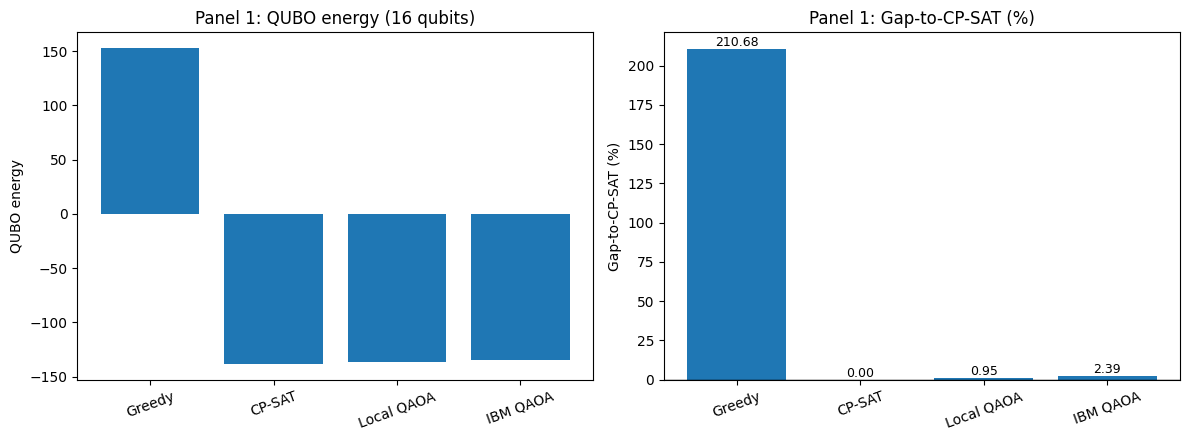
\includegraphics[width=0.92\textwidth]{images/panel1_results.png}
\caption{Validation panel. CP-SAT is the reference; Local QAOA and IBM QAOA remain within approximately $1\%$ of CP-SAT.}
\label{fig:panel1}
\end{figure}

\begin{figure}
\centering
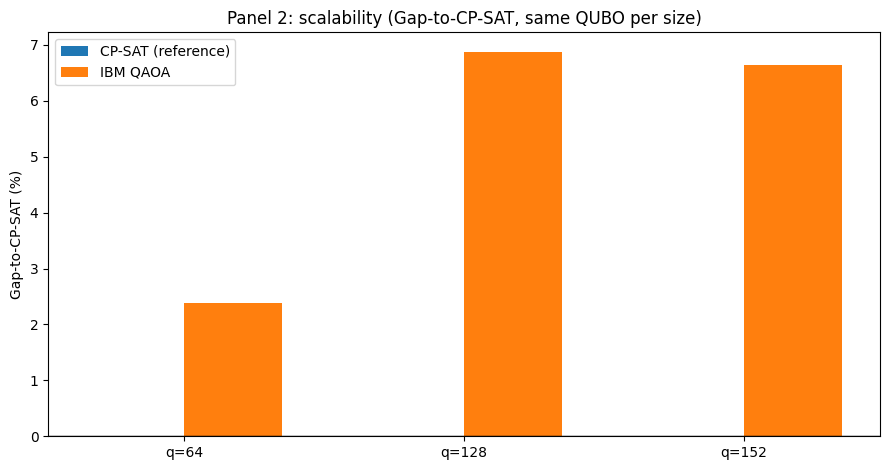
\includegraphics[width=0.92\textwidth]{images/panel2_results.png}
\caption{Scalability panel. IBM QAOA maintains a moderate gap to CP-SAT across hardware-scale instances.}
\label{fig:panel2}
\end{figure}

\section{Discussion}
\label{sec:discussion}

The validation results establish methodological consistency: with all methods on the same full QUBO and both QAOA variants within $1\%$ of CP-SAT, the quantum results are unlikely to be an artifact of a mismatched Hamiltonian, incorrect bit ordering, or an unfair metric. The scalability panel answers a different question---whether the proposed workflow remains feasible at hardware-relevant scales. These results do not constitute evidence of quantum advantage: CP-SAT remains a strong reference and QAOA uses a shallow $p=1$ circuit. Still, the IBM gap does not explode from 64 to 152 qubits, remaining within approximately $7\%$, which is meaningful because the quantum hardware executes a cybersecurity-inspired control QUBO rather than a synthetic benchmark problem. The gap-to-CP-SAT metric is central here, since raw QUBO energies scale with the number of variables and cannot be compared directly across sizes. The retained-coupling fractions ($60.09\%$ at 64 qubits, then $43.45\%$ and $46.43\%$) clarify the interpretation: the large-scale runs are hardware-feasibility demonstrations under a depth budget, not full-depth QAOA optimization of the dense Hamiltonian.

Several limitations follow from this design. CP-SAT is a reference under a finite time limit rather than a proof of optimality on the larger instances; QAOA is restricted to $p=1$, so higher depth might improve quality but would raise noise sensitivity, transpilation overhead, and barren-plateau risk~\cite{larocca2025barren}; the large-scale circuits optimize a pruned Hamiltonian even though all bitstrings are scored on the full QUBO; the formulation uses binary actions, with continuous or multi-level intensities requiring different encodings; and the implementation solves a single finite-horizon plan, leaving a receding-horizon deployment that repeatedly re-optimizes from the updated state to future work.

Despite these limitations, the study demonstrates the practical feasibility of solving cybersecurity-oriented optimization problems on current quantum hardware and provides a reproducible benchmark for future investigations of quantum-assisted cyber-defense mechanisms.

\section{Conclusion}
\label{sec:conclusion}

This paper presented a hybrid quantum--classical framework for cyber-defense optimization. The network is modeled through an extended state vector containing compromise, attacker knowledge, vulnerability exposure, and asset criticality, and a finite-horizon LQR-style objective is transformed exactly into a QUBO over binary defense actions, solved with Greedy, CP-SAT, Local QAOA, and IBM QAOA. Experimental results demonstrate that both Local QAOA and IBM QAOA produce solutions close to those obtained by the CP-SAT reference solver on the validation instance and maintain a moderate gap on larger hardware-scale problems. Although the results do not demonstrate quantum advantage, they demonstrate that a control-derived cyber-defense QUBO can be successfully executed on real IBM quantum hardware while preserving solution quality close to a strong classical benchmark. Future work will investigate receding-horizon control, improved QAOA parameter transfer, deeper but noise-aware circuits, error mitigation, and larger topologies with richer operational constraints. Therefore, the main experimentally supported claim of this work is that: IBM QAOA produces solutions comparable to a strong classical reference on validation instances and remains within a moderate gap on larger hardware-scale instances. From a cybersecurity perspective, the proposed framework introduces a systematic methodology for translating dynamic cyber-defense decision problems into optimization tasks suitable for both classical and quantum solvers.

\begin{thebibliography}{19}

\bibitem{miehling2019control}
Miehling, E., Rasouli, M., Teneketzis, D.: Control-theoretic approaches to cyber-security. In: Ba\c{s}ar, T., Zaccour, G. (eds.) Handbook of Dynamic Game Theory, pp.~1--27. Springer (2018)

\bibitem{rasouli2014supervisory}
Rasouli, M., Miehling, E., Teneketzis, D.: A supervisory control approach to dynamic cyber-security. In: Poovendran, R., Saad, W. (eds.) Decision and Game Theory for Security (GameSec 2014). Lecture Notes in Computer Science, vol. 8840, pp. 86--101. Springer, Cham (2014). \url{https://doi.org/10.1007/978-3-319-12601-2_6}

\bibitem{zhu2013game}
Zhu, Q., Ba\c{s}ar, T.: Game-theoretic approach to feedback-driven multi-stage moving target defense. In: Decision and Game Theory for Security, pp.~246--263. Springer (2013)


\bibitem{astafieva2025optimal}
Astafieva, M., Stepanenko, N.: Optimal cybersecurity management: Global controllability of linear models. In: CPITS~2025, CEUR-WS, vol.~3991, pp.~14--25 (2025)

\bibitem{nistcvss}
National Institute of Standards and Technology: National Vulnerability Database: Vulnerability Metrics. \url{https://nvd.nist.gov/vuln-metrics/cvss}

\bibitem{firstcvss}
Forum of Incident Response and Security Teams: Common Vulnerability Scoring System v4.0. \url{https://www.first.org/cvss/specification-document}

\bibitem{farhi2014qaoa}
Farhi, E., Goldstone, J., Gutmann, S.: A quantum approximate optimization algorithm. arXiv:1411.4028 (2014)

\bibitem{cerezo2021variational}
Cerezo, M., Arrasmith, A., Babbush, R., Benjamin, S.C., Endo, S., Fujii, K., McClean, J.R., Mitarai, K., Yuan, X., Cincio, L., Coles, P.J.: Variational quantum algorithms. Nature Reviews Physics 3, 625--644 (2021)

\bibitem{ortoolsdoc}
Google OR-Tools: CP-SAT Solver. \url{https://developers.google.com/optimization/cp/cp_solver}

\bibitem{perron2023cpsat}
Perron, L., Didier, F., Gay, S.: The CP-SAT-LP solver. In: CP~2023, LIPIcs, vol.~280, pp.~3:1--3:2 (2023)

\bibitem{lubinski2024optimization}
Lubinski, T., Coffrin, C., McGeoch, C., Sathe, P., Apanavicius, J., Bernal Neira, D.E.: Optimization applications as quantum performance benchmarks. ACM Transactions on Quantum Computing, Volume 5, Issue 3, Pages 1--44 (2024). https://doi.org/10.1145/3678184


\bibitem{barabasi1999scaling}
Barab\'asi, A.-L., Albert, R.: Emergence of scaling in random networks. Science 286(5439), 509--512 (1999)

\bibitem{bennett1984quantum}
Bennett, C.H., Brassard, G.: Quantum cryptography: Public key distribution and coin tossing. In: Proc. IEEE~Intl.\ Conf.\ on Computers, Systems and Signal Processing, pp.~175--179 (1984)


\bibitem{ibmquantum}
IBM Quantum: IBM Quantum Platform. \url{https://quantum.ibm.com}

\bibitem{zhang2025mtd}
Zhang, T., Kong, F., Deng, D., Tang, X., Wu, X., Xu, C., Zhu, L., Liu, J., Ai, B., Han, Z., Deng, R.H.:
Moving Target Defense Meets Artificial-Intelligence-Driven Network: A Comprehensive Survey.
IEEE Internet of Things Journal \textbf{12}(10), 13384--13397 (2025).
\url{https://doi.org/10.1109/JIOT.2025.3533016}

\bibitem{alarcon2026mtd}
Alarcon, A.I.D., Anaya, E.A., Duarte, N.A.C., Rodríguez, F.J.G.:
Rethinking Dynamic Security Strategies: A Survey of Moving Target Defense and Self-Defending Systems Design.
In: Mata-Rivera, M.F., Zagal-Flores, R. (eds.)
Telematics and Computing (WITCOM 2025).
Communications in Computer and Information Science, vol. 2704.
Springer, Cham (2026).
\url{https://doi.org/10.1007/978-3-032-09735-4_20}


\bibitem{pirani2022survey}
Pirani, M., Mitra, A., Sundaram, S.:
A Survey of Graph-Theoretic Approaches for Analyzing the Resilience of Networked Control Systems.
arXiv preprint arXiv:2205.12498 (2022).
\url{https://doi.org/10.48550/arXiv.2205.12498}

\bibitem{larocca2025barren}
Larocca, M., Thanasilp, S., Wang, S., et al.:
Barren Plateaus in Variational Quantum Computing.
Nature Reviews Physics \textbf{7}, 174--189 (2025).
\url{https://doi.org/10.1038/s42254-025-00813-9}

\bibitem{cherbal2024security}
Cherbal, S., Zier, A., Hebal, S., et al.:
Security in Internet of Things: A Review on Approaches Based on Blockchain, Machine Learning, Cryptography, and Quantum Computing.
Journal of Supercomputing \textbf{80}, 3738--3816 (2024).
\url{https://doi.org/10.1007/s11227-023-05616-2}

\bibitem{javadiabhari2024qiskit}
Javadi-Abhari, A., Treinish, M., Krsulich, K., Wood, C.J., Lishman, J.,
Gacon, J., Martiel, S., Nation, P.D., Bishop, L.S., Cross, A.W.,
Johnson, B.R., Gambetta, J.M.:
Quantum Computing with Qiskit.
arXiv preprint arXiv:2405.08810 (2024).
\url{https://doi.org/10.48550/arXiv.2405.08810}

\end{thebibliography}

\end{document}
